\documentclass[12pt,a4paper,fleqn]{article}
\title{Progress Report}
\author{Syed Ahmad Raza}
\date{2017.04.11}
\usepackage{mathtools}
\usepackage{graphicx}
\usepackage{color}          % for color eps output
\usepackage{afterpage}
\usepackage{newtxtext, newtxmath}

%\usepackage{layouts}       % for: \printinunitsof{in}\prntlen{\textwidth}

\begin{document}
	\maketitle
	\section*{\raggedright Numerical solution of Laplace equation using unequally spaced intervals}
    
    \subsection*{\raggedright Derivation of central difference formula for first \linebreak derivative with unequal intervals}
    
    Using the Taylor series expansion for a function $f(x)$ while neglecting second and higher order terms, we can write:
    \begin{equation} \label{eq:taylor1}
    f_{i+1} = f_i + f'_i(x_{i+1} - x_i) + \dots
    \end{equation}
    \begin{equation} \label{eq:taylor2}
    f_{i-1} = f_i - f'_i(x_i - x_{i-1}) + \dots
    \end{equation}
    Subtracting equation \eqref{eq:taylor2} from \eqref{eq:taylor1} gives:
    \begin{equation*}
    f_{i+1} - f_{i-1} \cong f'_i(x_{i+1} - x_{i-1})
    \end{equation*}
    \begin{equation} \label{eq:derivative1}
    f'_i = \frac{f_{i+1} - f_{i-1}}{x_{i+1} - x_{i-1}}
    \end{equation}
    
    \subsection*{\raggedright Derivation of central difference formula for second \linebreak derivative with unequal intervals}
    
    Now using the Taylor series expansion for the function $f(x)$ with second order terms but neglecting higher order ones, we have:
    \begin{equation} \label{eq:taylor3}
    f_{i+1} = f_i + f'_i(x_{i+1} - x_i) + f''_i\frac{(x_{i+1} - x_i)^2}{2!} + \dots
    \end{equation}
    \begin{equation} \label{eq:taylor4}
    f_{i-1} = f_i - f'_i(x_i - x_{i-1}) + f''_i\frac{(x_i - x_{i-1})^2}{2!} - \dots
    \end{equation}    
    Adding the above equations and rearranging gives:
    \begin{equation*}
    f''_i[(x_{i+1} - x_i)^2 + (x_i - x_{i-1})^2] \cong 2f_{i+1} + 2f_{i-1} - 4f_i - 2f'_i(x_{i+1} - 2x_i + x_{i-1})
    \end{equation*}
    \begin{equation*}
    f''_i = \frac{2(f_{i+1} - 2f_i + f_{i-1})}{(x_{i+1} - x_i)^2 + (x_i - x_{i-1})^2} - \frac{2f'_i(x_{i+1} - 2x_i + x_{i-1})}{(x_{i+1} - x_i)^2 + (x_i - x_{i-1})^2}
    \end{equation*}
    Substituting \eqref{eq:derivative1} in the above equation gives:
    \begin{equation} \label{eq:derivative2}
    f''_i = \frac{2(f_{i+1} - 2f_i + f_{i-1})}{(x_{i+1} - x_i)^2 + (x_i - x_{i-1})^2} - \frac{2(f_{i+1} - f_{i-1})(x_{i+1} - 2x_i + x_{i-1})}{(x_{i+1} - x_{i-1})[(x_{i+1} - x_i)^2 + (x_i - x_{i-1})^2]}
    \end{equation}
    
    \subsection*{\raggedright Discretization of Laplace equation for unequally spaced intervals}
    The following Laplace equation was considered:
    \begin{equation} \label{eq:laplace}
    \frac{\partial^2\phi}{\partial x^2} + \frac{\partial^2\phi}{\partial y^2} = 0
    \end{equation}
    For equally spaced intervals, this equation can be discretized as follows:
    \begin{equation} \label{eq:numlaplace1}
    \frac{\phi_{i+1,j}-2\phi_{i,j}+\phi_{i-1,j}}{(\Delta x)^2} +
    \frac{\phi_{i,j+1}-2\phi_{i,j}+\phi_{i,j-1}}{(\Delta y)^2} = 0
    \end{equation}
    For use in numerical solutions, equation \eqref{eq:numlaplace1} can be rearranged as follows:
    \begin{equation} \label{eq:numlaplace2}
    \phi_{i,j} = \left(
    \frac{\phi_{i+1,j}+\phi_{i-1,j}}{(\Delta x)^2} +
    \frac{\phi_{i,j+1}+\phi_{i,j-1}}{(\Delta y)^2}
    \right)\left(\frac{(\Delta x)^2(\Delta y)^2}{2[(\Delta x)^2+(\Delta y)^2]}\right)
    \end{equation}
    
    However, for unequally spaced intervals, equation \eqref{eq:derivative2} must be used to discretize each of the two terms in \eqref{eq:laplace} as follows:
    \begin{align} \label{eq:numlaplace3}
    &\frac{2(\phi_{i+1,j} - 2\phi_{i,j} + \phi_{i-1,j})}{(x_{i+1} - x_i)^2 + (x_i - x_{i-1})^2} - \frac{2(\phi_{i+1,j} - \phi_{i-1,j})(x_{i+1} - 2x_i + x_{i-1})}{(x_{i+1} - x_{i-1})[(x_{i+1} - x_i)^2 + (x_i - x_{i-1})^2]} + {} \nonumber\\
    &\frac{2(\phi_{i,j+1} - 2\phi_{i,j} + \phi_{i,j-1})}{(y_{j+1} - y_j)^2 + (y_j - y_{j-1})^2} - \frac{2(\phi_{j+1} - \phi_{j-1})(y_{j+1} - 2y_j + y_{j-1})}{(y_{j+1} - y_{j-1})[(y_{j+1} - y_j)^2 + (y_j - y_{j-1})^2]} \nonumber\\
    &= 0
    \end{align}
    Rearranging the above equation for use in numerical solutions:
    \begin{align*}
    &\frac{2(\phi_{i+1,j} + \phi_{i-1,j})}{(x_{i+1} - x_i)^2 + (x_i - x_{i-1})^2} - \frac{2(\phi_{i+1,j} - \phi_{i-1,j})(x_{i+1} - 2x_i + x_{i-1})}{(x_{i+1} - x_{i-1})[(x_{i+1} - x_i)^2 + (x_i - x_{i-1})^2]} \\
    &{} + \frac{2(\phi_{i,j+1} + \phi_{i,j-1})}{(y_{j+1} - y_j)^2 + (y_j - y_{j-1})^2} - \frac{2(\phi_{j+1} - \phi_{j-1})(y_{j+1} - 2y_j + y_{j-1})}{(y_{j+1} - y_{j-1})[(y_{j+1} - y_j)^2 + (y_j - y_{j-1})^2]} \\
    &= \frac{4\phi_{i,j}}{(x_{i+1} - x_i)^2 + (x_i - x_{i-1})^2} + \frac{4\phi_{i,j}}{(y_{j+1} - y_j)^2 + (y_j - y_{j-1})^2}
    \end{align*}
    \begin{align*}
    &\phi_{i,j} = \\
    &\left[\frac{2(\phi_{i+1,j} + \phi_{i-1,j})}{(x_{i+1} - x_i)^2 + (x_i - x_{i-1})^2} - \frac{2(\phi_{i+1,j} - \phi_{i-1,j})(x_{i+1} - 2x_i + x_{i-1})}{(x_{i+1} - x_{i-1})[(x_{i+1} - x_i)^2 + (x_i - x_{i-1})^2]} + {} \right.\\
    &\left.\frac{2(\phi_{i,j+1} + \phi_{i,j-1})}{(y_{j+1} - y_j)^2 + (y_j - y_{j-1})^2} - \frac{2(\phi_{j+1} - \phi_{j-1})(y_{j+1} - 2y_j + y_{j-1})}{(y_{j+1} - y_{j-1})[(y_{j+1} - y_j)^2 + (y_j - y_{j-1})^2]}\right]\\
    &\times\frac{1}{4}\left[\frac{1}{(x_{i+1} - x_i)^2 + (x_i - x_{i-1})^2} + \frac{1}{(y_{j+1} - y_j)^2 + (y_j - y_{j-1})^2}\right]^{-1}
    \end{align*}
    \begin{align} \label{eq:numlaplace4}
    &\phi_{i,j} = \nonumber\\
    &\left[\frac{2(\phi_{i+1,j} + \phi_{i-1,j})}{(x_{i+1} - x_i)^2 + (x_i - x_{i-1})^2} - \frac{2(\phi_{i+1,j} - \phi_{i-1,j})(x_{i+1} - 2x_i + x_{i-1})}{(x_{i+1} - x_{i-1})[(x_{i+1} - x_i)^2 + (x_i - x_{i-1})^2]} + {} \right.\nonumber\\
    &\left.\frac{2(\phi_{i,j+1} + \phi_{i,j-1})}{(y_{j+1} - y_j)^2 + (y_j - y_{j-1})^2} - \frac{2(\phi_{j+1} - \phi_{j-1})(y_{j+1} - 2y_j + y_{j-1})}{(y_{j+1} - y_{j-1})[(y_{j+1} - y_j)^2 + (y_j - y_{j-1})^2]}\right] \nonumber\\
    &\times\frac{1}{4}\left[\frac{[(x_{i+1} - x_i)^2 + (x_i - x_{i-1})^2][(y_{j+1} - y_j)^2 + (y_j - y_{j-1})^2]}{(x_{i+1} - x_i)^2 + (x_i - x_{i-1})^2 + (y_{j+1} - y_j)^2 + (y_j - y_{j-1})^2}\right]
    \end{align}
    For the case of equally spaced intervals when
    \begin{align*}
    &(x_{i+1} - x_i) = (x_i - x_{i-1}) = 0\text{ ,}\\
    &(y_{j+1} - y_j) = (y_j - y_{j-1}) = 0\text{ ,}\\
    &(x_{i+1} - 2x_i + x_{i-1}) = 0\text{ and}\\
    &(y_{j+1} - 2y_j + y_{j-1}) = 0\text{ ,}
    \end{align*}
    then equation \eqref{eq:numlaplace4} reduces to equation \eqref{eq:numlaplace2}.
    \subsection*{Unequal grid coordinates}
    A $100\times100$ grid was selected with the following functions for the x and y axes:
    \begin{equation} \label{eq:xcoordinates}
    f(x)=\frac{L}{2}\left[ 1 + \sin\left(\pi\left(\frac{i}{n_x} -
    \frac{1}{2}\right)\right)\right]
    \end{equation}
    \begin{equation} \label{eq:ycoordinates}
    f(y)=W\sin\left(\frac{\pi}{2}\times\frac{j}{n_y}\right)
    \end{equation}
    The resulting grid and the graphs of its functions are shown in the figure below.
    \begin{figure}
        \centering
        \includegraphics[width=\linewidth]{../figures/gridAndGraph.eps}
        \caption{The selected grid with the chosen $x$ and $y$ functions and their graphs}
        \label{fig:gridandgraphs}
    \end{figure}
    
    \subsection*{SOR Method}
    For equal grid intervals, Successive Over-Relaxation (SOR) method applied to Laplace equation was as follows:
    \begin{equation} \label{eq:numlaplacesorequal}
    \phi^{m+1}_{i,j} = (1-\omega)\phi^m_{i,j} + \omega
    \left(
    \frac{\phi^m_{i+1,j}+\phi^{m+1}_{i-1,j}}{(\Delta x)^2} +
    \frac{\phi^m_{i,j+1}+\phi^{m+1}_{i,j-1}}{(\Delta y)^2}
    \right)\left(\frac{(\Delta x)^2(\Delta y)^2}{2(\Delta x^2)(\Delta y^2)}
    \right)
    \end{equation}
    For unequal grid intervals, SOR method can be applied to Laplace equation using equation \eqref{eq:numlaplace4} as follows:
    \begin{align} \label{eq:numlaplacesorunequal}
    &\phi^{m+1}_{i,j} = (1-\omega)\phi^m_{i,j} + \omega\times{} \nonumber\\
    &\left[\frac{2(\phi^m_{i+1,j} + \phi^{m+1}_{i-1,j})}{(x_{i+1} - x_i)^2 + (x_i - x_{i-1})^2} - \frac{2(\phi^m_{i+1,j} - \phi^{m+1}_{i-1,j})(x_{i+1} - 2x_i + x_{i-1})}{(x_{i+1} - x_{i-1})[(x_{i+1} - x_i)^2 + (x_i - x_{i-1})^2]} + {} \right.\nonumber\\
    &\left.\frac{2(\phi^m_{i,j+1} + \phi^{m+1}_{i,j-1})}{(y_{j+1} - y_j)^2 + (y_j - y_{j-1})^2} - \frac{2(\phi^m_{j+1} - \phi^{m+1}_{j-1})(y_{j+1} - 2y_j + y_{j-1})}{(y_{j+1} - y_{j-1})[(y_{j+1} - y_j)^2 + (y_j - y_{j-1})^2]}\right] \nonumber\\
    &\times\frac{1}{4}\left[\frac{[(x_{i+1} - x_i)^2 + (x_i - x_{i-1})^2][(y_{j+1} - y_j)^2 + (y_j - y_{j-1})^2]}{(x_{i+1} - x_i)^2 + (x_i - x_{i-1})^2 + (y_{j+1} - y_j)^2 + (y_j - y_{j-1})^2}\right]
    \end{align}
    
    This equation was solved using $\omega = 1.8$ for a $100\times100$ grid. After $1,114$ iterations, the numerical solution stopped changing, according to the following formula:
    \begin{equation} \label{eq:tolerance}
    \text{max}\Big(|\phi^{m+1}_{i,j} - \phi^m_{i,j}|\Big) \leq 1\times 10^{-9}
    \end{equation}
    
    The error between the numerical solution and the exact solution is shown below in the figure.
    
    \begin{figure}[!b]
    \centering
    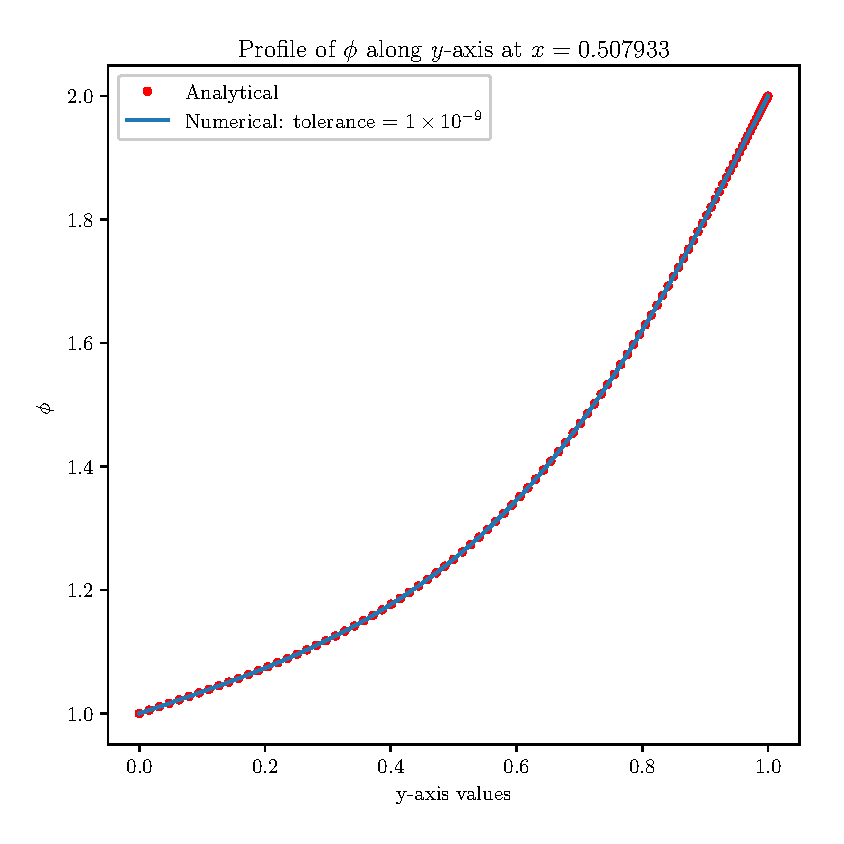
\includegraphics[width=\linewidth]{../figures/laplaceUnequalConvergence.eps}
    \caption{Comparison of numerical solution and exact solution of Laplace
    equation with unequal grid intervals}
    \label{fig:errorcomparison}
    \end{figure}
    
    \section*{Further work in progress}
    \subsection*{\raggedright Numerical solution of 2D Navier-Stokes equation}
    Following is the Navier-Stokes equation:
    \begin{equation}
    \frac{\partial u}{\partial t} + \frac{\partial (uu)}{\partial x} + \frac{\partial (uv)}{\partial y} = -\frac{1}{\rho}\frac{\partial P}{\partial x} + \nu \left(\frac{\partial^2u}{\partial x^2} + \frac{\partial^2u}{\partial y^2}\right)
    \end{equation}
    Navier-Stokes equation has to be solved numerically for a 2D problem using SOR method for pressure term and upwind scheme for the convective term, with Dirichlet boundary conditions at the inlet and walls and Neumann boundary condition on the exit.
    
\end{document}